\chapter{Design of Adaptivity}
\label{chap:design-of-adaptivity}

In the last chapter, we have mentioned how we incorporated many of the
strategies to support learning and motivation into the game.
In this chapter, we discuss another strategy which helps to achieve the state of
flow, the one that is special to ALS  % TODO:reformulate
-- recommending tasks of optimal difficulty.
% ... "which is the secret sauce of adaptive learning systems"
% ... "which is powered by the AI"
% TODO: More links to learning/motivation \label{sec:motivation.challenge}
% TODO: link to the adaptivity chapter

\section{Expected Behavior}  % or "Specification", "Goals", "System Behavior", "Behavior specification"
\label{sec:robomission.behavior}

% NOTE: This section should provide a useful basis for:
% - guide how to design ALS components
% - setting rewards for a a RL/planning agent
% - defining "good recommendations" (~good performance) for supervised
%   learning and for use in monitoring/evaluation (domain metric)

% TODO: clarify the relationship between this section and AL.analysis (or
% possibly also this-chapter.analysis) sections.

Wide range of task difficulties, combined with the adaptive behavior,
should make the system useful for anybody who wants to learn
introductory programming.
However, this long-term goal requires many iterations and a lot of data.
Currently, the system primarily targets at children 10-15 years old.
% "between 10 and 15 years."

The main use case of the system is a 1-2 hours in-classroom tutorial
(``Hour of Code'' style), with a possible follow-up individual practice at home.
In line with the system mission (\cref{sec:mission}), goals of this tutorial
are to teach the student basic concepts of programming,
help them to spend most of the time in the state of flow,
and motivate them for the further learning of computer science.
% TODO: better link to fullfilling human needs (as stated in table in chapter 2)
% TODO: better terminoglogy, because "You cannot motivate people... (motivation
% goes fron inside)"
% NOTE: flow is a goal; but at the same time it supports the other 2 goals

After each solved task, the student is shown a dialog window with one
recommended task, and with a link to the page with overview of all tasks.
% Terminology: \emph{good recommendation}
Ideally, each recommendation should lead to the state of flow.
% TODO: How to measure? One way: looking ath the long-term objectives
As we cannot directly observe whether the student is in the state of flow,
we must rely on proxy data, which can be either subjective
(using perceived difficulty ranking),
or objective (using observed performance), %should be neither too low, nor too high),
% "qualitative" vs. "quantitative"
% TODO: REF:performance
as we have discussed in section
on attributable metrics (\cref{sec:live-evaluation}).
% long-term or attributable metrics \cref{sec:long-term-objectives,sec:live-evaluation}
% TODO: the performance compression should be described in this chapter
% in student modeling section, ideally with an analysis supporting the
% decsions or sketching some possible directions.

% TODO: Reformulate: (e.g. why is it useful, useful for what)
Unfortunately, both subjective and objective approach to measure flow
is very noisy. Therefore, it is useful to formulate weaker, but better observable
requirements on the system behavior:
% NOTE: It reminds me of hypothesis testing of goodness-of-fit: there are
% various tests (metrics we can measure), that can tell us, that the given
% sample is definitely not from the compared distribution; some of these
% tests are very simple and intuitive (e.g. for exp. distribution, ratio
% of mean and stdev^2 should be 1), but they also have quite small power
% (i.e. they are often not able to reject false hypotheses).
% TODO: shrink vertical spaces
\begin{itemize}
\item The student is able to solve any task recommended by the system, ideally
  in a reasonable time (20 minutes).
    Furthermore, the student is able to solve the first few tasks quickly
    (in 2 minutes) and progress to the second level quickly (in at most 10
    minutes).
\item The best performing students (supposedly with a prior programming skill)
should progress through a first few levels quickly, spending at most 5 minutes
on tasks practicing only sequences of commands, and get to the more
challenging tasks containing both types of loops and conditional statements
in at most 20 minutes.  % 10, 15?
\item All students should gradually start practicing all basic programming concepts
  (sequence, loops, conditional statements) during the first hour of the tutorial.
  % TODO: check gvid
\item Average difficulty of the recommended tasks should gradually increase.
  (Occasionally, an easy tasks might be recommended in order to improve
  exploration, but these easy tasks should
  not be too frequent, and they should be differentiated for the student,
  e.g. as \emph{speed challenges} in order to explain the sudden change in
  difficulty.)
\item At most one new programming concept and one new game concept should appear
  in a task. No new concept should be introduced, until the student
  solves at least one task with the last introduced concept with a good
  performance. % (they must sometimes come together, it is not a problem)
% TODO: perform analysis if it's the case in the current system.
%Each new concept (e.g. block) is explained in the task where it appears for the first time. (REF: img), so the student understands all elements in the game world and blocks available in the toolbox.
\item If asked after each task, students should report that the task was
  neither too easy, nor too difficult for them in at least half of the tasks
  during the tutorial.  % or another negative tag, such as boring, weird, ...
\item Neither task that was reported as too easy should take them
  more than 1 minute, and there should never be more then 3 too easy tasks
  in a row (with the exception of the first level).
  %(Student is not bored by neither too easy task requiring many commands (i.e.
  %taking more than 1 minute to build the streightforward solution), nor by the
  %sequence of either too easy or too similar tasks.
  % TODO: Maybe it would be better to state it in combined max too-easy time?
  % NOTE: It is ok to have sometimes an easy task (esp. at the beginning), but
  % they should be quick to solve and not too frequent
\item If asked at the beginning and at the end of the tutorial about their
  interest in learning computer science, the end report should be statistically
  higher.
% TODO: Not sure if to mention the self-report points, as they are not
% currently used in the system.
% TODO: (Another flow-related) If the student marks the current task as too
% easy, the next task is strictly more difficult. If the student marks the
% current task as too difficult, the next task is as most as difficult as the
% current one.
\end{itemize}
% TODO: compare these requiremnts againts collected data and gvid-report



%\subsection{Main Use Case}
%\label{sec:robomission.use-case}
%
%\begin{itemize}
%\item Student visits the home page of the project, reads the "promotional slides" and tries the game with manual controls. On the last slide, they click on the recommended task from the 1st level.
%(REF: img)
%\item Student creates the program using Blockly blocks and can run the program as many times as needed. (REF: img) Program execution is visualized. Student can change the speed of the execution.
%\item After each unsuccessful execution, a short message explaining why the task was not solved is shown (e.g. "The spaceship must reach the final row.") (REF: img)
%\item Student is able to solve the first few tasks quickly (within 2 minutes).
%\item After solving each task, student is shown a visualization of obtaining points (called credits) (REF: printscreen). After a few solved tasks, student progresses to next level.
%\item After each solved task, student is shown a dialog with one recommended task, and also a link to the page with overview of all tasks (REF: img).
%\item Student is able to solve any task recommended by the system (within 15 minutes).
%\item Each new concept (e.g. block) is explained in the task where it appears for the first time. (REF: img), so the student understands all elements in the game world and blocks available in the toolbox.
%\item Students with some prior programming skill should progress through first few levels quickly (within 10 minutes) and get to the more challenging tasks containing both types of loops, conditionals etc.
%\item Student is not bored by neither too easy task requiring many commands (i.e. taking more than 1 minute to build the streightforward solution), nor by the sequence of either too easy or too similar tasks.
%\item Student can sign up (or log in without registration through their social accounts) at any moment to save their progress. Even without singing up, the system can associate the student with its progress using session cookie (but also provides a button to clear the history).
%\item Student can provide a feedback or report a bug easily (and the feedback is send to admins by an email).
%\end{itemize}
%(TBA: add diagram with images for all these steps linked by arrows showing transitions)

% TODO: consider some of the following notes
% - Design of tasks for the system is described in section \ref{sec:robomission.tasks}.
% - Adaptive aspect of the behavior is described in section \ref{sec:robomission.adaptability}.
%\item intuitive and simple user interface crucial (aiming at children, they need to focus on learning programming, it would be bad to waste their mental power on understanding a complex interface)
%\item mini-instructions (ref to the Google research on ignoring instructions, show how it was solved in Blockly Games; ref figure)
%\item mini-explations (difference from instructions: after the fact) (ref figure) (they also serve as a convenient mean to game resetting)
%\item motivation: intrinsic (fun challenging game + optimal difficulty) and simple external motivation scheme: credits and levels


%\subsection{Four Modes of Usage}
%\label{sec:robomission.use-cases}
%
%In addition to the main use case described in the previous section,
%which assumes a new student without any context (e.g. a classroom),
%the system can be potentially used in other (or more specific) ways.
%
%\begin{itemize}
%\item "Hour of Code" mode
%  \begin{itemize}
%  \item single hour
%  \item mainly as a motivation to programming
%  \item using RoboBlocks
%  \item directly at elemenatry and high schools, or at home
%  \item plus: MjUNI workshop
%  \item shorter promotianal version for DODs (?) ("10 minutes of code")
%  \item (should be strictly time-limited; certificate at the end)
%  \end{itemize}
%\item "Foundations mode" individual learning of elementary programming (individual at home or in a classroom, from several days to several weeks, depending on the prior skill); natural continuation of the first "Hour of Code" (next levels, with RoboBlocks)
%\item "University mode" -- levels with RoboCode/Python, at home / secondary schools, KSI (0th problem set), IB111 (0th/1st motivational lesson - needs Python and to be better than turtle)
%\item "Competition mode" -- competitions such as Purkiada, Pevnost FI, KSI
%(advanced problem sets), new FIBot (physical version already in InterSoB 2017,
%then in Sob 2018); this also includes testing mode for RH interns
%\end{itemize}
%
%All these modes can be naturally implemented as distinct levels,
%going from the easy tasks using RoboBlocks for "Hour of Code",
%gradually transitioning to the RoboCode during learning the "Foundations",
%using full-fledged Python for "University mode"
%and offering both blocks and Python for the individual competitions.
%Levels from the past competitions can be made public for all students.


\section{Domain Model}

%In this phase of development, we have decided not to model overlapping concepts,
% NOTE: not enough data, not clear how they combine and how they relate to PS
% which are still needed for the users
Currently, we do not model overlapping concepts, since their use would require
more data to analyze their interaction.
Instead, we devide tasks into disjoint linearly order hierarchical problem
sets (\cref{fig:robomission.domain}). % , which are easier to handle.
% ... We started by manually dividing tasks into 9 problem sets (levels)
The hierarchy has two levels: the top-level problem sets are call \emph{missions},
and they contain about 8-10 tasks, which are further split into three smaller
problem sets called \emph{phases}.
Missions and phases are ordered, while tasks within a given phase are not.
The missions were chosen primarily by the available programming blocks and
included game elements, and secondarily by an estimated difficulty.
% (initialy human-estimated, later refined using collected data
% NOTE: Data collected befor division into phases (TODO: mention in the
% analysis chapter...)
The contribution of refining the missions into phases is threefold:
\begin{itemize}
\item Phases enforce important prerequisities within a mission (e.g.
introducing wormholes before using them in more difficult tasks).
\item Phases help to achieve a balanced composition \cite{progression-analysis},
  introducing new concepts in the first phase,
  recombining them with previously learned concepts in the second phase,
  and further reinforcing (practicing) of known concepts in the third phase.
% TODO: Although this division is only a guide, doesn't hold exatly...
% TODO: elaborate on the relevance of the paper
% TODO: check the paper (terms of the phases, their "oreder" and meaning)
%The resulting two-level hierarchical and ordered problem set structure is shown
%in \cref{fig:robomission.domain}.
\item Phases are approximately homogeneous, i.e. difficulty of all tasks in a
  given phase is similar. This allows allows for simpler tutor models.
  % and they practic similar concepts
\end{itemize}
% TODO: link to what presented in earlier chapters

\begin{figure}[htb]
\centering
TODO: domain diagram\\
(all 9 missions with labels; unlabeled nodes for phases and tasks)
% should show covered concepts: sequences of commands, repeat, while, if, if-else, simple tests (comparing)
\caption{Domain model used in RoboMission.}
\label{fig:robomission.domain}
\end{figure}


\section{Student Model}

% TODO: terminology and links from \cref{sec:student-modeling}
For each student we keep track of her skill for each problem set. % phase and mission.
The skill $s \in [0, 1]$ represents manifested ability to solve tasks in
a given problem set. The initial skill is 0, it is increased after each solved
task from the problem set, and once the skill reaches 1 the problem set is solved.
The model is decsriptive, because it does not model the probability of
a student solving a task (with some performance), but rather an amount
of verified skill.
An advantage is that this skill can be shown directly to the student
(e.g. visualized as a progressbar towards completion of the current mission).
% E.g. at the beginning, the probability is higher than 0 for sure.
% used directly in visualization

We use discrete representation of performance with 3 levels (poor, good,
excellent). Currently, only solving time is considered for the performance
compression: for each task, we set a time threshold for a solution to be
considered as good or excellent
(set as 1.5 and 0.75 multiples of median time).
% TODO: support the decision by an analysis (REF)
% TODO: Note that it's huge simplification and a subject of future research.

After each solved task session, the corresponding skill is increased by
an amount $p \in [0, 1]$ which depends on the performance.
For each performance level, we set the increment such that $1/p$ tasks solved
with such performance are enough for manifesting mastery in this phase.
The increment does not depend on the task, because we assume homogeneous
phases.  %, and it does not depend on our previous estimate
Either a single task solved with an excellent performance, or two
tasks solved with a good performance are enough to solve the phase,
translating into $p_{excellent} = 1$ and $p_{good} = 0.5$.
Furhtermore, solving all tasks in a phase (even if with a poor performance),
should be always enough to solve the phase.
%(this is a technical requirement, stemming from the fact that we do not want
%to present students with the same task they already solved again)
Therefore, the update rule is:
$s \leftarrow \min(1, s + \max(p, \frac{1}{n}))$,
where $n$ is the number of tasks in the phase.
% The $1/n$ term ensures that the student eventually masters the phase.
% NOTE: we never want to decrease skill of a student

To aggregate the skills of the phases into the skill of the mission,
we simply take average of the phase skills.
In future, we would like to use more sohpisticated aggregation,
which would allow to compensate unsolved tasks in the first phase
by more difficult tasks in the later phases.
% TODO: reformulate

\section{Tutor Model}

We currently focus on the outer-loop tutor modeling.
Concerning the inner loop, the system provide only a basic
rule-based agent for displaying instructions and explanations,
as described in \cref{sec:game.explanations}.

The outer-loop tutor is hierachical;
it first selects a problem set, then a task from this problem set.
In order to assess if a problem set is mastered,
the corresponding verified skill
computed by the student model described in the previous section
is compared to the threshold of 1. % ?
% TODO: diagram of PS, TS selection and mastery decison

The tutor selects for practice the first unmastered phase of the first
unmastered mission, using the total ordering provided by the domain model.
The system contains only a small number of problem sets,
so it is reasonable to assume that the student would like to solve all of
them,
% TODO: further increased by the tendency to "get everything green"
in which case it is preferable to solve them in the order from the
easiest to the most difficult.
Homogenity of phases allow to safely select a task uniformly at random from
all unsolved tasks in that phase, which is a strategy maximizing exploration.
% UI:
Recommendations provided by the system are \emph{soft};
i.e. that student can ignore them and select any task
from the overview of all tasks.

Progression through the missions and phases gradually increases the difficulty,
but the increase is not monotonous.
% TODO: Reformulate not to use so many "increase"
Perceived difficulty increases after progess to a new phase,
but it decreases during solving tasks from the same phase,
as the student's skill improves, while the objective difficulty stays
approximately same (\cref{fig:robomission.flow}).
On one hand, it means that the difficulty does not always match student's
skills perfectly, possibly slightly overshooting at the beginning of a phase,
and undershooting at the end.
On the other hand, it means that the perceived difficulty level is not
same all the time, but has a wavy character, which is more interesting
for students % \emph{dramaturgy of flow}
\cite{book-of-lenses}.

\begin{figure}[htb]
\centering
TODO: flow diagram specifically for progress through phases
(increase of challenge with each new phase, then constant during the phase)
% result: waves, but more "spiky"
% (but the objective difficulty does not decrease, it stays constant
% (so it's important to think what is on the y-axis!)
\caption{Dramaturgy of flow in RoboMission.}
\label{fig:robomission.flow}
\end{figure}



% TODO? UI? Probably not enough material for this



\section{Analysis Layer}
\label{sec:robomission.analysis-layer}

In order to iteratively improve adaptivity, as well as the programming game
and other aspects of the ALS,
an analysis layer (\cref{sec:metrics-and-evaluation})
that provides several different views on the behavior of the system
is crucial.
Our analysis layer includes the following components:

% \subsection{Monitoring Components}
%To fulfill the requirements from section \ref{sec:admin-requirements},
%the system includes the following components:

\begin{itemize}
\item \emph{Google Analytics}
  shows distribution of users with respect to the time and space.
  In addition to page visits,
  it can also process specific events sent from the frontend
  (such as clicking on the execution button),
  and divide them into groups, e.g. by the task being solved
  % or group for AB experiment.
  (\cref{fig:google-analytics}).
\item \emph{Monitoring Dashboard}
  shows values of a few long-term objectives % metrics related to the long-term objectives
  %(\ref{sec:long-term-objectives})
  in the last month, namely daily active students, daily solved tasks, and
  solving hours (total time spent on successful attempts)
  (\cref{fig:monitoring-dashboard}).
  % + "success ratio" = proportion of successful attempts,
  The system also computes a few metrics for each task
  (solved count, median time, and success ratio) in order to detect
  bugs in them.
  % These metrics are recomputed every night.
\item \emph{Monitoring Notebook}
  is a weekly-recomputed jupyter notebook (CITE) that performs several analyses
  and visualizations using the latest data (\cref{fig:monitoring-notebook}).
  It serves the similar purpose as the monitoring dashboard, but it is
  easier to extend. It is enough to add a cell into the notebook;
  %and test it on a collected data,
  no change to the backend or frontend is needed.
  %NOTE: + investigation notebook that with a command that generates exports
  %and serves them directly as pandas data frames
\item \emph{Error Reports and User Feedback}.
  If an unhandled top-level error occurs on the server,
  it is not only logged, but also sent to the administrators.
  Administrators also receive emails with messages provided by users via
  a feedback form that can be invoked on any page.
\item \emph{Data Exports and Logs}.
  All collected data are exported every week as a zip bundle containing
  CSV files prepared for %convenient offline analysis.
  offline analysis.
  In addition, all requests, performed actions, and unhandled errors % and submitted feedbacks
  are logged to text files on the server for manual inspection.
\end{itemize}


\imgW{google-analytics}{%
  Preview from Google Analytics (January--March 2018).} % (breakdown for "execution" event).}

% TODO: make it readable or remove
\imgW{monitoring-dashboard-fragment}{%
  Number of active students and number of solved tasks during March 2018
  visualized in the monitoring dashboard.}

% TODO: check if the table lines looks ok when printed
\begin{figure}[htb]
\centering
\begin{subfigure}{.48\textwidth}
\centering
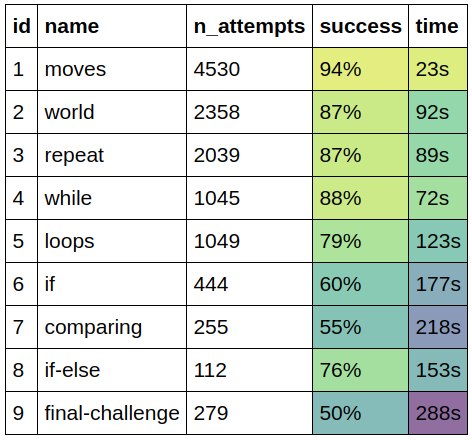
\includegraphics[width=0.95\textwidth]{img/monitoring-notebook-levels}
\end{subfigure}
\begin{subfigure}{.51\textwidth}
\centering
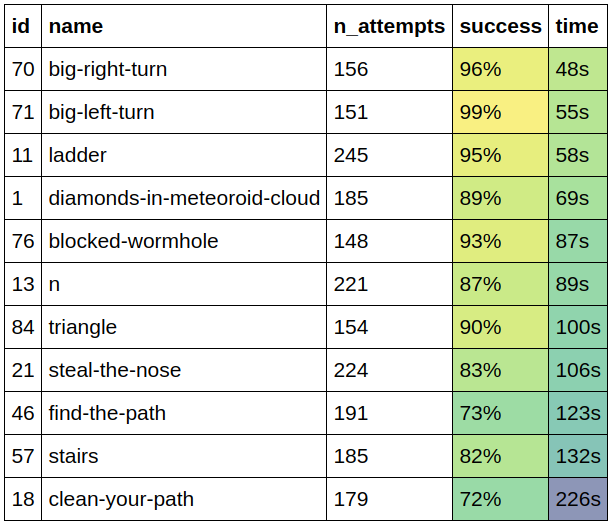
\includegraphics[width=0.95\textwidth]{img/monitoring-notebook-repeat}
\end{subfigure}
\caption{%
  Mean success and median time for all missions (left),
  and tasks in the Repeat mission (right),
  visualized in the monitoring notebook
  from March 31, 2018. This simple analysis reveals e.g.
  that 7th mission (comparing) is probably more difficult than the 8th (if-else),
  % it's not clear, because the population of students is different; they
  % might already learn something important in the 7th level for the 8th
  % level
  and that Clean Your Path task is significantly more difficult than
  the other tasks in the mission.}
% TODO: observation about clean-your-path
\label{fig:monitoring-notebook}
\end{figure}

% TODO: update investigation notebook (fix error in last cell, current data;
% should show something interesting, or at least some descriptive analylis)
%\imgW[0.7]{investigation-notebook}{Template of jupyter notebook for investigation of live data.}



% NOTE on iterative development: first prototype: 2016, one year of
% development, thrown away; for testing our initial ideas and find what works
% and what not; 50 tasks with a robot in maze; problems with the robot in the
% maze: not fun (boring, not inovative, repetitiveness), did not allow for a
% plenty of diverse easy tasks (which is necessary for adaptive systems),
% required a lot of blocks even for simple programs (compared to the SpaceGame)
% + problems with the codebase (maintainability, extensibility - why?); and the
% good things? (SPA, explored/verified useful technologies, such as Blockly and
% Django)

%\imgW{prototype-task-environment}{First prototype of the system, with a classic robot-in-maze game.}


%\subsection{Admin Requirements}
%\label{sec:admin-requirements}
%Similarly to regular users, administrators also have requirements on the systems:
%\begin{itemize}
%\item Admin can immediately see how much is the system used and how the system behaves with respect to the short-term ("live-evaluation") metrics (...)
%\item Admin receives feedback from provided by users, and error reports on unhandled exceptions.
%\item Admin can see metrics on individual tasks (to quickly detect issues with a task).
%\end{itemize}


% TODO: consider if to include non-functional requirements or not
%\section{Non-functional Requirements}
%\label{sec:robomission.nonfunctional-requirements}
%
%\begin{itemize}
%\item easy to understand code, pleasure to read and write (extend)
%\item easy to refactor and add new things (new tasks, levels, recommendation strategies etc.)
%\item robust, efficient, interpretable behavior
%\end{itemize}
